% original version by:  Nikos Drakos, CBLU, University of Leeds
% * revised and updated by:  Marcus Hennecke, Ross Moore, Herb Swan
% * with significant contributions from:
%   Jens Lippmann, Marek Rouchal, Martin Wilck and others 
%%\title{ibs}


\chapter{Intra-Beam Scattering}
\label{chap:IBS}

The Intra-Beam Scattering command computes the contribution to emittance
growth rates due to Coulomb scattering of particles within relativistic
beams. The algorithms in this module have been derived from the formalism
presented in 1982 by J.D.~Bjorken and S.K.~Mtingwa
[\href{../Introduction/bibliography.html#bm1}{Bjorken and Mtingwa}], 
and are also using the expansion of M. Conte and M. Martini
[\href{../Introduction/bibliography.html#conte}{Conte and Martini}]
developped in 1985,  generalized to the case of nonzero vertical
dispersion.  

The present implementation of the IBS module in \madx is described in a
forthcoming note  [Antoniou and Zimmermann] (2012).   

The syntax of the \texttt{IBS} command is:
\madbox{
%IBS, TOLERANCE=real, STEPS=integer, FILE=string;
IBS, FILE=string;
}

The \texttt{IBS} command has one attribute:
\begin{madlist}
%  \ttitem{TOLERANCE} ??? (Default:~1.e-7) % declared, never used
%  \ttitem{STEPS} number of steps ??? (Default:~50) % declared, never used
  \ttitem{FILE} outputs the resulting "ibs" table to
  the named file. (Default:~"ibs")
\end{madlist}

The Bjorken-Mtingwa formalism takes into account the variation of the
lattice parameters (beta and dispersion functions) around the
machine and consequently, the knowledge of the optical functions along
the machine is required: \texttt{IBS} should only be called after fully
qualified \texttt{BEAM} command and a \texttt{TWISS} command. 

{\bf Warning:} Calling \texttt{EMIT} between the \texttt{TWISS} and
\texttt{IBS} commands leads to \texttt{IBS} using wrong beam parameters,
even if the \texttt{BEAM} command is reiterated.

The \texttt{IBS} module does not include a consistent treatment of
linear betatron coupling.   

The intra-beam scattering growth times are given by:
%%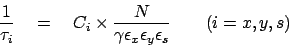
\includegraphics{img1.png}
\[
 \frac{1}{\tau_i} \quad = \quad C_i \times \frac{N}{\gamma \epsilon_x
   \epsilon_y \epsilon_s} \qquad (i = x, y, s) 
\]
where $C_i$ accounts for some constants and the integrals for the
scattering functions, N is the number of particles in the bunch,
$\gamma$ is the relativistic factor and $\epsilon_i$ are the normalized
emittances in the horizontal, vertical and longitudinal plane
respectively. These key beam parameters must be specified through the
\texttt{BEAM} command. 

If the \texttt{CENTRE=true} option of \texttt{TWISS} was specified,
the optical functions are calculated by \texttt{TWISS} at the center of 
each element and \texttt{IBS} uses these values for the element. 
If by default \texttt{TWISS} calculated the optical functions at the end
of each element, \texttt{IBS} calculates the values at the center of
each element by performing a linear interpolation between the end values
for the previous element and the end values for the current element.

  
{\bf Input of the beam parameters:}\\
A number of parameters have to be present in the  \texttt{BEAM} command
in order to run the IBS module: 

\begin{madlist}
  \ttitemn{PARTICLE} This is mandatory but \madx provides default
  value of \texttt{PARTICLE=proton}. For ions, this parameter specifies
  only the name of the ions, and the MASS (approximated to the atomic
  unit number times the neutron mass \texttt{NMASS}) and CHARGE must be
  provided as well.

  \ttitemn{NPART} the number of particles (or number of ions).

  \ttitemn{ENERGY} The definition of the energy (total, kinetic, total
  energy of the ions or energy per nucleon) is a difficult one. In the
  present approach, the energy is the \textbf{total} energy of the
  particle. For ions, the expected input is the \textbf{proton
    equivalent} energy, i.e. the total energy a proton would have when
  circulating in the defined machine. As an illustration, in the LHC,
  protons will be injected with an energy of 450 GeV. Consequently, to
  evaluate the growth times for Lead ions at injection in the LHC, one
  has to input \texttt{ENERGY=450*charge}. \\
  An important check for the correctness of the input is the printed value
  of the relativistic factor  $\gamma$. The latter should correspond to:   
  %%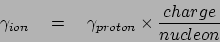
\includegraphics{img5.png}
  \[
  \gamma_{ion} \quad = \quad \gamma_{proton} \times \frac{charge}{nucleon}
  \]

  \ttitemn{emittances} This part of the input is used to define the
  normalized horizontal, vertical and longitudinal emittances. 
  The required parameters are the \texttt{physical} transverse
  emittances, \texttt{EX} and \texttt{EY}, and the longitudinal
  emittance \texttt{ET}.\\  
  The longitudinal emittance is defined  as the product of the bunch
  length \texttt{SIGT} times the relative energy spread \texttt{SIGE},
  which are therefore required input. \\  
  If only the longitudinal emittance is defined, and \texttt{SIGT}
  and \texttt{SIGE} are omitted, an active RF cavity is also
  necessary in the lattice to infer \texttt{SIGT} and \texttt{SIGE}.

\end{madlist}


{\bf Example of BEAM input:}\\
A beam of fully stripped Lead ions at the LHC injection energy may be
defined as follows for \texttt{IBS} calculations: 
\madxmp{
nucleon = 208; \\
charge = 82; \\
\\
BEAM, \=PARTICLE= lead, CHARGE= charge, MASS= nucleon*nmass, \\
      \>ENERGY= 450*charge, NPART= 1.1E7, BUNCHED, \\
      \>EX= 7.82E-9, EY= 7.82E-9, SIGE= 4.68E-4, SIGT= 0.115;
}


{\bf Resulting Table and File:} \\
The IBS command produces a table "ibs" containing the following data for
each element of the machine: element name, position, optical functions
(beta, alfa, dispersion and derivative) in both transverse planes, as
well as the particular variables DELS, the length difference in meters
between consecutive elements, and TXI, TYI and TLI, the IBS growth times
in the two transverse and longitudinal planes. 

This table can be accessed through the usual mechanisms, and if the
attribute \texttt{FILE="file\_name"} was given, \madx writes this table
to the named file.  



{\bf Features:} \\
The average growth rates in [sec] are defined as variables called
\texttt{ibs.tx}, \texttt{ibs.ty}, \texttt{ibs.tl} for the horizontal,
vertical and longitudinal growth times respectively. They are directly
accessible as variables after the \texttt{IBS} command, e.g.
\madxmp{
IBS; \\ 
Tx = ibs.tx;}   
defines a variable Tx which is the average horizontal growth rate in seconds. 



{\bf Examples:} \\
The two examples provided for the module Intra-Beam Scattering
illustrate the commands required to run the module. The two examples
have been selected such as to highlight the differences between a
computation for protons and that for ions. Both examples compute the IBS
growth times at injection into the LHC. The examples are located
\href{http://madx.web.cern.ch/madx/madX/examples/ibs/}{here}.

% Frank Schmidt 2003-05-23 
% Ghislain Roy 2014-08-07

%% EOF
